\documentclass[a4paper]{article}


\usepackage{alphabeta} 
\usepackage{enumitem} 
\usepackage{mathtools}
\usepackage{amsmath, amssymb} 
\usepackage{amsthm}
\usepackage{cancel} 
\usepackage[margin=0.70in]{geometry} 
\geometry{left=3cm,right=3cm,top=2.4cm,bottom=2.4cm}	%the page geometry as defined, A4=210x297mm
\usepackage{graphicx}
\usepackage{wrapfig}
\usepackage[center]{caption}
\usepackage{textcomp}
\usepackage{tabto}
\usepackage{layout}
\usepackage{bm}
\usepackage{minipage-marginpar}
\usepackage[dvipsnames]{xcolor}
\usepackage{hyperref}
\usepackage{dutchcal}
\usepackage{derivative}
\usepackage{esint}
%\usepackage{biblatex}
\usepackage{subcaption}
\usepackage{booktabs}\usepackage{derivative}
\usepackage[flushleft]{threeparttable}
\usepackage[capbesideposition=outside,capbesidesep=quad]{floatrow}
\usepackage{derivative}
\usepackage[thinc]{esdiff}
\usepackage{lipsum}
\usepackage{arydshln}
%%RENEW

\newtheorem{problem}{Άσκηση}
\newtheorem*{solution*}{Λύση}
\newtheorem{definition}{Ορισμός}[subsection]
\newtheorem{properties}{Ιδιότητες}[subsection]
\newtheorem{theorem}{Θεώρημα}[subsection]
\newtheorem{protash}{Πρόταση}[subsection]
\newtheorem{porisma}{Πόρισμα}[subsection]
\newtheorem{lemma}{Λήμμα}[subsection]
\newtheorem*{prooof}{Απόδειξη}
\newtheorem*{notes}{Παρατηρήσεις}
\newtheorem*{note}{Παρατήρηση}
\newtheorem*{app}{Εφαρμογή} 
\newtheorem*{example}{Παράδειγμα}
\newtheorem*{examples}{Παραδείγματα}


\newcommand\numberthis{\addtocounter{equation}{1}\tag{\theequation}}
%\renewcommand{\labelenumi}{\roman{enumi}}
\newcommand{\approxtext}[1]{\ensuremath{\stackrel{\text{#1}}{\approx}}}
\renewcommand{\figurename}{Εικόνα.}
\renewcommand{\tablename}{Πίνακας.}
%\renewcommand\refname{New References Header}
\renewcommand*\contentsname{Περιεχόμενα}
%\DeclareDerivative{\odv}{\mathrm{d}}


\begin{document}
\begin{titlepage}			%makes a title page. Remember to change the author, CID, username and group number to what is appropriate for you!
	\centering
	{\scshape\LARGE Εθνικό Μετσόβιο Πολυτεχνείο\par}
	{\scshape \LARGE Σ.Ε.Μ.Φ.Ε.\par}
	\vspace{1cm}
	{\huge\bfseries Μέτρηση της φωτοαγωγιμότητας του CdS συναρτήσει της έντασης και της συχνότητας της ακτινοβολίας διέγερσης\par}
	\vspace{1cm}
	{\Large\itshape Θωμόπουλος Σπύρος\par}		%remember to change these!
	
	%		{\large Group \@group\unskip\strut\par}
	{\large spyros.thomop@gmail.com/ ge19042@mail.ntua.gr\par \hfill \\}% 		%remember to change these!
	\vspace{1cm}
	{\large Ημερμονηνία Παράδοσης 23/05/2022\par}
\end{titlepage}

\subsection*{Σκοπός}
	
	Ο στόχος της εν λόγω εργαστηριακής άσκησης είναι ο υπολογισμός της καμπύλης ρεύματος-τάσης, της φωτοαγωγιμότητας και την εξάρτησή της από την ένταση και την συχνότητα της προσπίπτουσας ακτινοβολίας, για έναν φωτοαντιστάτη από CdS. Η διέγερση του CdS θα πραγματοποιηθεί μέσω ΗΜ ακτινοβολίας στο ορατό.
	
\subsection*{Θεωρητικά Στοιχεία}

	Η \textit{φωτοαγωγιμότητα} πρόκειται για το φαινόμενο κατά το οποίο αυξάνεται η αγωγιμότητα ενός ημιαγώγιμου υλικού κατά την απορρόφηση ΗΜ ακτινοβολίας. Σε έναν ημιαγωγό το ενεργειακό χάσμα μεταξύ της Ζώνης Σθένους(ΖΣ) και της Ζώνης Αγωγιμότητας(ΖΑ) είναι $<4eV$, έτσι όταν προσπέσει σε αυτόν ακτινοβολία μεγαλύτερης ή ίσης ενέργειας, διεγείρει τα ηλεκτρόνια από την ΖΣ στην ΣΑ και εμφανίζονται κενά ηλεκτρονίων, δηλαδή ''θετικά'' φορτισμένες οπές στην ΖΣ. Εξ' αιτίας της διατήρησης της ορμής επιβάλλει μόνο τις διεγέρσεις μεταξύ ίδιων κυματανυσμάτων $\vec{k}$.
	
	Καθώς αυξάνεται η ενέργεια της προσπίπτουσας ΗΜ ακτινοβολίας, τα ηλεκτρόνια καταλαμβάνουν ολοένα υψηλότερες ενεργειακά στάθμες της ΖΑ, επομένως θα αυξάνεται και συντελεστής απορρόφησης
	\begin{align*}\label{1}
		\alpha = L(hv-E_g)^{1/2},\hspace{0.8cm}\text{L:σταθερά,$hv\geq E_g$} \numberthis
	\end{align*}
	
	 
	
	Γενικότερα, θα έχουμε κίνηση τόσο των ηλεκτρονίων όσο και των οπών και σε αυτή την κίνηση οφείλεται η αγωγιμότητα του ημιαγωγού. Συγκεκριμένα, αν n και p οι συγκεντρώσεις των ηλκετρονίων και των οπών αντίστοιχα, $\mu_e,\mu_h$, η ευκινησία τους, δηλαδή το πόσο γρήγορα μπορούν να κινηθούν εντός του ημιαγωγού όταν εφαρμοστεί ηλεκτρικό πεδίο, τότε θα είναι	
	\begin{align*}\label{2}
		\sigma = \sigma_e + \sigma_p = ne\mu_e + pe\mu_h = ne(\mu_e+\mu_p) \numberthis
	\end{align*}

	Διεγέρσεις ηλεκτρονίων μπορούμε να έχουμε με δύο τρόπους. Ο πρώτος είναι θερμικά, με ρυθμό μετάβασης $g_0$ και ο δεύτερος, όπως έχει ήδη αναφερθεί, είναι μέσω ακτινοβολίας με ρυθμό $g$ και κάθεμία από αυτές συνεισφέρει στην αγωγιμότητα, ενώ αντίστοιχα έχουμε και επανασυνδέσεις ηλεκτρονίων-οπών. Αν λάβουμε υπόψιν μας και τον χρόνο $\tau_n$ που απαιτείεται για να επέλθει η ισορροπία, τότε προκύπτει το ότι η φωτοαγωγιμότητα είναι 
	\begin{align}\label{3}
		\sigma_{ph} = \frac{\alpha(\omega)I(\omega)e\tau_n(\mu_e+\mu_h)}{\hbar \omega}
	\end{align}
	
	Από την σχέση (\ref{1}) έχουμε ότι η προσπίπτουσα ακτινοβολία πρέπει να ικανοποιεί την συνθήκη $E_{in}=hv\geq E_g$, δηλαδή η ενέργειά της να είναι μεγαλύτερη ή ίση από το ενεργειακό κενό προκειμένου να έχουμε την απορρόφησή της από τα ηλεκτρόνια της ζώνης σθένους, άρα φωτοαγωγιμότητα. Όμως, όταν η ενέργεια είναι πολύ μεγαλύτερη από το ενεργειακό κενό $E_g$, τότε θα έχουμε το ότι ο συνελεστής απορρόφησης γίνεται πολύ μεγάλος και η ακτινοβολία απορροφάται στην επιφάνειά του. Εκεί υπάρχουν ατέλειες που συνεισφέρουν στην επανένωση ηλεκτρονίων-οπών, άρα την μείωση του $\tau_n$, άρα την μείωση της φωτοαγωγιμότητας αφού είναι ανάλογη του $\tau_n$. 
	
	Γενικά θα έχουμε τρεις περιοχές διαφορετικής συμπεριφοράς της φωτοαγωγιμότητας ανάλογα με το μήκος κύματος.
	\begin{itemize}
		\item[.] \textit{Περιοχή Ι  :} Έχουμε μικρό μήκος κύματος και κυριαρχούν τα παραπάνω φαινόμενα στην επιφάνεια, δηλαδή μικρή φωτοαγωγιμότητα \vspace{-0.2cm}
		\item[.] \textit{Περιοχή ΙI :} Πρόκειται για την μεσαία περιοχή όπου η παρουσιάζεται το μέγιστο της φωτοαγωγιμότητας  \vspace{-0.2cm}
		\item[.] \textit{Περιοχή ΙII:} Έχουμε μεγάλα μήκη κύματος και ασθενή απορρόφηση, άρα μικρή φωτοαγωγιμότητα
	\end{itemize}

\subsection*{Πειραματική Διάταξη}
	Η πειραματική διαδικασία, άρα και η διάταξη χωρίζεται σε δύο μέρη.
	\subsubsection*{Α Μέρος}
		Εδώ, η διάταξη αποτελείται από: 
			\begin{itemize}
				\item[.] Πηγή λευκού φωτός \hspace{-0.2cm}
				\item[.] Συγκλίνων φακός   \hspace{-0.2cm}
				\item[.] Σχισμή για τον περιορισμό του φωτός από την πηγή \hspace{-0.2cm}
				\item[.] Φακός ευθυγράμμισης \hspace{-0.2cm}
				\item[.] Πολωτής \hspace{-0.2cm}
				\item[.] Αναλυτής \hspace{-0.2cm}
				\item[.] Συγκλίνων φακός με $f=15cm$ \hspace{-0.2cm}
				\item[.] Φωτοαντιστάτης από CdS \hspace{-0.2cm}
				\item[.] Ηλεκτρικό κύκλωμα στο οποίο συνδέεται ο φωτοαντιστάτης CdS  το οποίο αποτελέιται επιπλέον από μία πηγή συνεχούς, μία αντίσταση 1Ω συνδεδεμένη παράλληλα με τον φωτοαντιστάτη, ένα αμπερόμετρο και ένα βολτόμετρο
			\end{itemize}
			Με τον πολωτή και τον αναλυτή μπροούμε να ελέγξουμε την ένταση της τελικής δέσμης που θα καταλήξει στο CdS χρησιμοποιώντας τον ν.Malus
			\begin{align}\label{4}
				I = I_0cos^\theta
			\end{align}
			
			Η διάταξη φαίνεται στην Εικόνα (\ref{im1})
				\begin{figure}[h!]
					\centering
					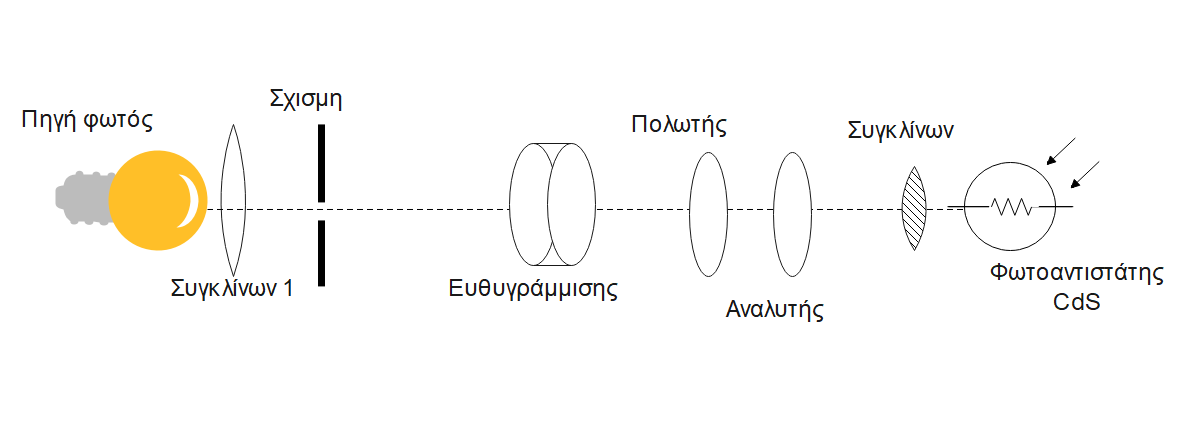
\includegraphics[scale=0.5]{part1.png}
					\caption{Διάταξη Α Μέρους}
					\label{im1}
				\end{figure}
				
			
	\subsubsection*{B' Μέρος}
		H διάταξη του Β Μέρους αποτελείται από
			\begin{itemize}
			\item[.] Πηγή λευκού φωτός\vspace{-0.2cm}
			\item[.] Συγκλίνων φακό\vspace{-0.2cm}
			\item[.] Σχισμή για τον περιορισμό του φωτός από την πηγή  \vspace{-0.2cm}
			\item[.] Φακός ευθυγράμμισης \vspace{-0.2cm}
				\item[.] Πρίσμα για να αναλύσουμε την δέσμηη του φωτός \vspace{-0.2cm}
				\item[.]  Περιστρεφόμενος δρομέας για να τοποθετηθεί το πρίσμα \vspace{-0.2cm}
				\item[.]  Γωνιόμετρο\vspace{-0.2cm}
				\item[.] Σχισμή για την απομόνωση μικρού εύρους μηκών κύματος\vspace{-0.2cm}
							\end{itemize}
	Η διάταξη φαίνεται στην Εικόνα (\ref{im2})
	
		\begin{figure}[h!]
			\centering
		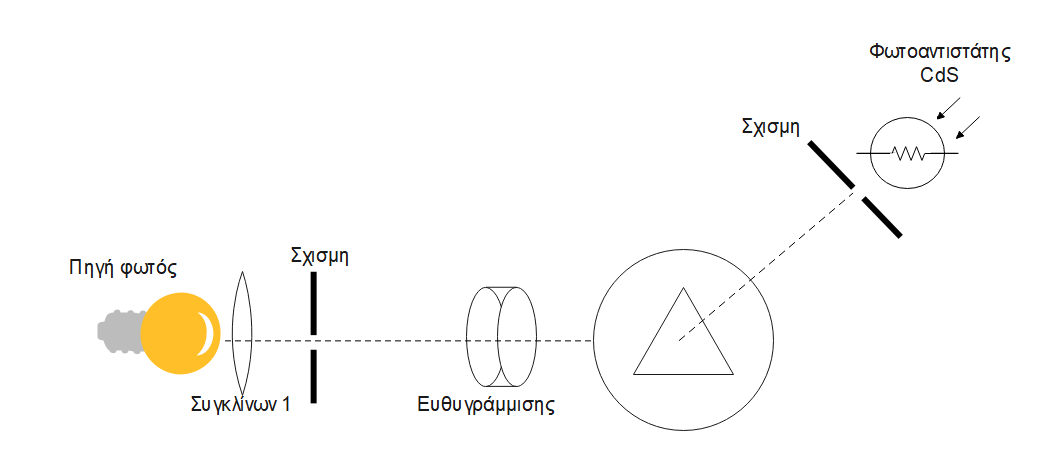
\includegraphics[scale=0.3]{part2.png}
		\caption{Πειραματική Διάταξη Β Μέρους}
		\label{im2}
		\end{figure}
	
	
\subsection*{Πειραματική Διαδικασία - Επεξεργασία Μετήσεων }

	\subsubsection*{Α Μέρος: Καμπύλη Φωτορεύματος-Τάσης}
		Αφού συναρμολογήσουμε την διάταξη της Εικόνας (\ref{im1}), παίρνουμε σταθερές θέσεις έτσι ώστε να μην επηρεάζεται η ένδειξη για το φωτορευμα με την μεταβολή της φωτεινότητας του τριγύρω χώρου ανάλογα με τις αλλαγές στην θέση μας. Τώρα, για κάθε τιμή της τάσης στα άκρα του CdS $V=\{20,15,9,3\}V$ και για γωνίες του πολωτή $\theta=\{0,20,50,70,90\}^o$ μετράμε το ρεύμα που προκύπτει από την φωτοαγωγιμότητα του CdS. Σε κάθε αλλαγή της τάσης μετράμε και το ρεύμα που προκύπτει από το υπόβαθρο, προκειμένου να το αφαιρέσουμε από την τιμή που μετρήσαμε με την πηγή φωτός ανοιχτή. Τα αποτελέσματα φαίνονται στον παρακάτω Πίνακα (\ref{mat1})
		
%		\begin{table}[h!]
%			\centering
%			\begin{tabular}{r|r||r|r||r|r|r}
%			V(V) & $I_{back}(mA)$ & $I(0)(mA)$ & $I(20)(mA)$&$I(50)mA$&$I(70)(mA)$&$I(90)(mA)$\\\hline\hline
%					20&0.010&\underline{0.044}&\underline{0.037}&2.103&\underline{0.079}&0.078\\
%15&0.008&3.040&2.759&1.544&0.577&0.063\\
%9&0.004&1.748&1.586&0.899&0.352&0.037\\
%3&0.001&0.572&0.520&0.299&0.115&0.012
%			\end{tabular}
%     
%			\begin{tabular}{r|r||r|r||r|r}
%	V(V) & $I_{true}(0)$& $I_{true}(20)$& $I_{true}(50)$& $I_{true}(70)$& $I_{true}(90)$\\ \hline\hline		
%	20&\underline{0.034}&\underline{0.027}&2.093&\underline{0.069}&0.068\\
%15&3.032&2.751&1.536&0.569&0.055\\
%9&1.744&1.582&0.895&0.348&0.033\\
%3&0.571&0.519&0.298&0.114&0.011
%			\end{tabular}
%			
%			\caption{ }
%			\label{mat1}
%		\end{table}

\begin{table}[h!] 
	\centering
	\begin{tabular}{r|r|r|r|r}
	V(V) & $I_{back}(mA)$ & $I(0)(mA)$ & $I(15)mA$ & $I(45)m(A)$ \\\hline\hline
	20& 0.040& 9.00& 8.10& 5.20\\
	18& 0.035& 7.80& 7.50& 4.70\\
	15& 0.027& 6.60& 6.20& 3.90\\
	9 & 0.020& 3.80& 3.60& 2.35\\
	6 & 0.011& 2.70& 2.60& 1.68
	\end{tabular}
	
	\begin{tabular}{r|r|r|r}
		$V(V)$ & $I_{true}(0)(mA)$ & $I_{true}(15)(mA)$ & $I_{true}(45)(mA)$ \\\hline\hline	
		20&8.96&8.06&5.16\\
		18&7.76&7.465&4.665\\
		15&6.573&6.173&3.873\\
		 9&3.78&3.58&2.33\\
		 6&2.689&2.589&1.669
	\end{tabular}
	\caption{ }
	\label{mat1}
\end{table}
		
\vspace{-0.5cm}		
Οι γραφικές παραστάσεις Φωτορεύματος-Τάσης για τις διαφορετικές τιμές της γωνίας $\theta$ του αναλυτή φαίνονται στην Εικόνα (\ref{im3}) και έχουν προκύψει από την μέθοδο των ελαχίστων τετραγώνων. 		
	
	\begin{figure}[h!]
		\centering
		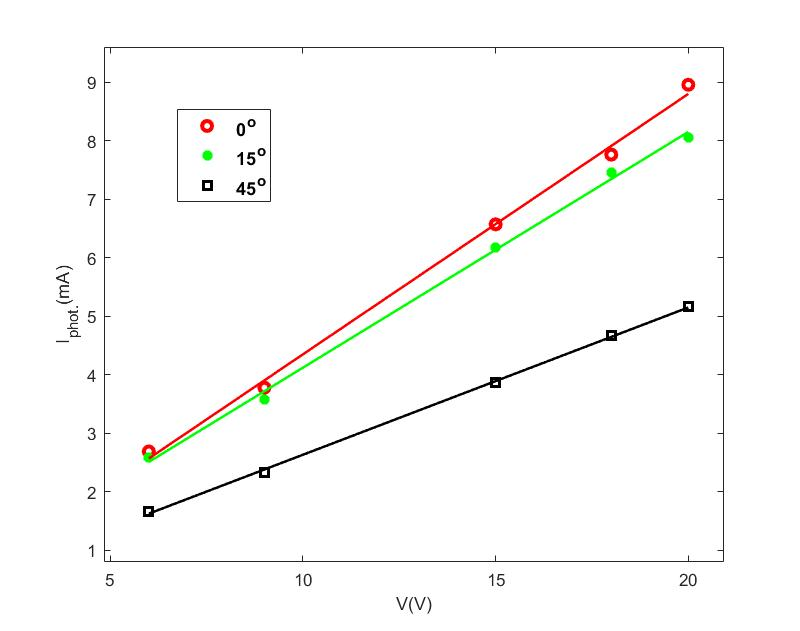
\includegraphics[scale=0.31]{plot1.jpg}	
		\caption{ }
		\label{im3}
	\end{figure}			
		
%Έχω αγνοήσει τις τιμές του φωτορεύματος που φαίνονται υπογραμμισμένες στον Πίνακα (\ref{mat1}).
		
Η κλίση κάθε ευθείας που προκύπτει από την μέθοδο ελαχίστων τετραγώνων αντιστοιχεί στην εκάστοτε τιμή της αγωγιμότητας $\sigma$. Όλες οι τιμές φαίνονται στον Πίνακα (\ref{mat2})		
	\begin{table}[h!]
		\centering
		\begin{tabular}{r|r|r}
			$\theta$ & $\sigma_{\theta}(10^{-4}\Omega)$ & $cos^2\theta$\\\hline\hline
			0        & 0.45		& 1.000	\\
			15       & 0.40     & 0.933 \\
			45       & 0.25     & 0.500 \\
		\end{tabular}	
	\caption{ Αγωγιμότητα συναρτήσει της $\theta$.}		
	\label{mat2}
	\end{table}
		
		Η γραφική παράσταση $cos^2\theta - \sigma_{\theta}$ φαίνεται στην Εικόνα (\ref{im3b}) όπου παρατηρούμε ότι η αγωγιμότητα εξαρτάται γραμμικά από το $cos^2\theta$ που σημαίναι ότι από τον ν.Malus (\ref{4}) θα εξαρτάται γραμμικά και από την ένταση του εισερχόμενου φωτός.
		\begin{figure}[h!]
			\centering
			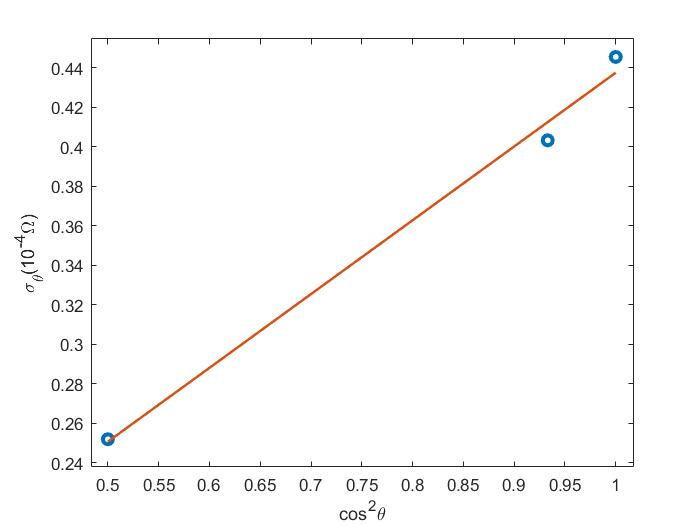
\includegraphics[scale=0.45]{plot2.jpg}
			\caption{$cos^2\theta-\sigma_\theta$ }
			\label{im3b}
		\end{figure}
		
		Η γραμμικότητα είναι εμφανής από την παραπάνω γραφική παράσταση και με την επιβεβαίωσή της, επιβεβαιώνουμε πως φωτοαγωγιμότητα και ένταση προσπίπτουσας ακτινοβολίας είναι ευθέως ανάλογες
		
		
	\subsubsection*{B' Μέρος}
	
		Στο Μέρος Β, θα μελετήσουμε την εξάρτηση του φωτορεύματος από το μήκος κύματος της προσπίπτουσας ακτινοβολίας. Τροφοδοτούμε το κύκλωμα του φωτοαντιστάτη με $V=30V$ και παρατηρούμε το φάσμα της λάμπας που έχει αναλυθεί από το πρίσμα. Τώρα μετράμε τις γωνίες στις οποίες βρίσκεται το ερυθρό και το ιώδες του φάσματος, οι οποίες αντίστοιχα είναι $\phi_{\epsilon} = 140^o$ και 
		$\phi_{\iota}=144^o $.
 Τώρα μεταβάλλουμε την γωνία κατά $0.5^o$ από $\phi_{\epsilon}$ εως
      $\phi_{\iota}$ και μετράμε το αντίστοιχο φωτόρευμα. Τα αποτελέσματα φαίνονται στον Πίνακα (\ref{mat3}).
      
		\begin{table}[h!]
			\centering
			\begin{tabular}{r|r|r}
				 $\theta_n(^o)$ & $ I_0(\mu A)$ & $I_{back}(\mu A)$ \\\hline\hline
				144.0& 1.10& 0.70\\
				143.5& 1.22& 0.85\\
				143.0& 1.41& 0.93\\
				142.5& 1.65& 0.96\\
				142.0& 2.11& 0.98\\
				141.5& 2.36& 1.10\\
				141.0& 3.11& 1.10\\
				140.5& 2.39& 1.11\\
				140.0& 2.10& 1.13
			\end{tabular}
			\caption{ }
			\label{mat3}
		\end{table}
		
		Θεωρώντας γραμμική την σχέση γωνίας-μήκους κύματος, δηλαδή $\lambda(nm)=\alpha_0\phi+\beta_0$ και γνωρίζοντας τις γωνίες που αντιστοιχούν στα δύο άκρα του ορατού που είναι $\lambda_{\epsilon}=700nm$ και $\lambda_{\iota} = 400nm$, μπορούμε να βρούμε τις σταθερές, οι οποίες προκύπτουν: $\alpha_0 = -75[nm]$, $\beta_0=11200[nm]$, άρα 
		\begin{align}\label{5}
			\lambda[nm] = -75\phi[^o] + 11200 
		\end{align}
		
		Κατ' επέκταση, από την σχέση $E = hc/\lambda$ μπορούμε να υπολογίσουμε την ενέργεια της ακτινοβολίας που αντιστοιχεί σε κάθε γωνία. Επίσης, η πηγή ακτινοβολεί διαφορετική ένταση για κάθε μήκος κύματος σύμφωνα με τον ν.Planck:
		\begin{align}\label{6}
			F(\lambda ,T) = \frac{2\pi hc^2}{\lambda^5(exp(hc/\lambda kT ) - 1 )}
		\end{align}
		
		Τώρα, θα πρέπει να κανονικοποιήσουμε την τιμή του καθαρού φωτορεύματος με έναν συντελεστή $\alpha_{norm}=F/F_{max}$. Τα αποτελέσματα φαίνονται στον Πίνακα (\ref{mat4}): 
		\begin{table}[h!]
			\centering
			\begin{tabular}{r|r|r|r|r|r|r}
			$\theta(^o)$ & $I_{\kappa\alpha\theta}(\mu A)$ & $\lambda(nm)$ & $F_n(\lambda,T)(10^{13}W/m^3)$ & $ E(eV)$ & $\alpha_{norm}$ & $I'_{\text{κανον.}}(mA)$ \\\hline\hline
	144.0 &0.40 & 400.0 & 0.602 & 3.10 & 0.389 & 0.16 \\
	143.5 &0.37 & 437.5 & 0.811 & 2.83 & 0.525 & 0.19 \\
	143.0 &0.48 & 475.0 & 1.009 & 2.61 & 0.653 & 0.31 \\
	142.5 &0.69 & 512.5 & 1.181 & 2.42 & 0.765 & 0.53 \\
	142.0 &1.13 & 550.0 & 1.320 & 2.25 & 0.855 & 0.97 \\
	141.5 &1.23 & 587.5 & 1.424 & 2.11 & 0.922 & 1.16 \\
	141.0 &2.01 & 625.0 & 1.493 & 1.98 & 0.967 & 1.94 \\
	140.5 &1.28 & 662.5 & 1.532 & 1.87 & 0.991 & 1.27 \\
	140.0 &0.97	& 700.0 &	1.545 &	1.77 & 1.000 & 0.97 \\
			\end{tabular}
			\caption{Όπου $T=4.13\times10^3K$ }
			\label{mat4}
		\end{table}
		
		Από τον Πίνακα (\ref{mat4}) παίρνω την παρακάτω γραφική E-$I_{norm}$:
			\begin{figure}[h!]
				\centering
				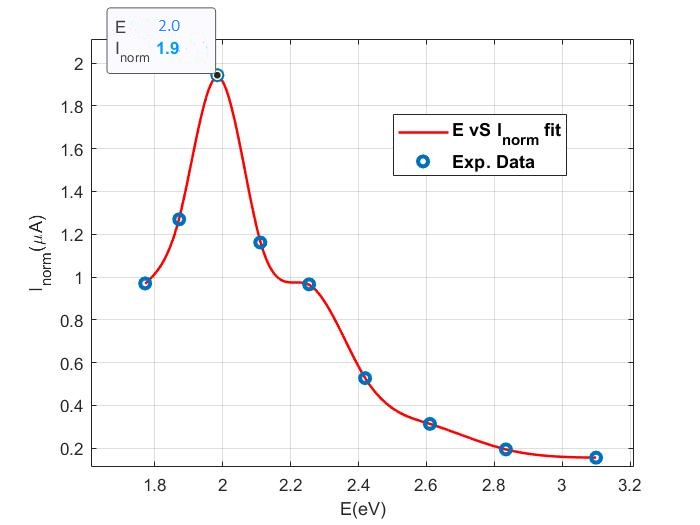
\includegraphics[scale=0.7]{plot4.jpg}
				\caption{ }
				\label{im4}				
			\end{figure}
			
			
		Φαίνεται πως η καμπύλη είναι αντίστοιχη με την θεωρητική, δηλαδή ότι παρουσιάζει ένα μέγιστο φωτόρευμα και οι υπόλοιπες τιμές είναι μικρότερες. Το ζήτημα είναι πως ενώ περιμέναμε να παρουσιάζεται στα $2.4eV$, εδώ φαίνεται ότι προκύπτει στα 2.0eV, δηλαδή έχουμε σψετικό σφάλμα της τάξης του $\sim17\%$, το οποίο είναι πολύ μεγάλο.
		
\subsection*{Συμπεράσματα}

		Τα σφάλματα εν γένει ήταν μεγάλα και αισθητά και στα δύο μέρη της διαδικασίας. Ενδεχομένως να οφείλονται στην πολυκαιρία των οργάνων αλλά επίσης και στο γεγονός ότι δεν είχαμε πλήρη συσκότιση με αποτέλεσμα η παραμικρή μετατόπισή μας εντός του χώρου να επιφέρει διαφορετική τιμή στις μετρήσεις.
		
\end{document}